\chapter{Introduction}

Over the last few decades, the rate of obesity and overweight people in the World has greeatly increased. As presented for the UK case in the figure \ref{fig:obesity_uk}, the obesity rate has increased by 12 \% between 1980 and 2013, and by 13 \% for the overweight rate. It is forecasted by the World Health Organisation to continue to grow.

\begin{figure}[h]
    \centering
    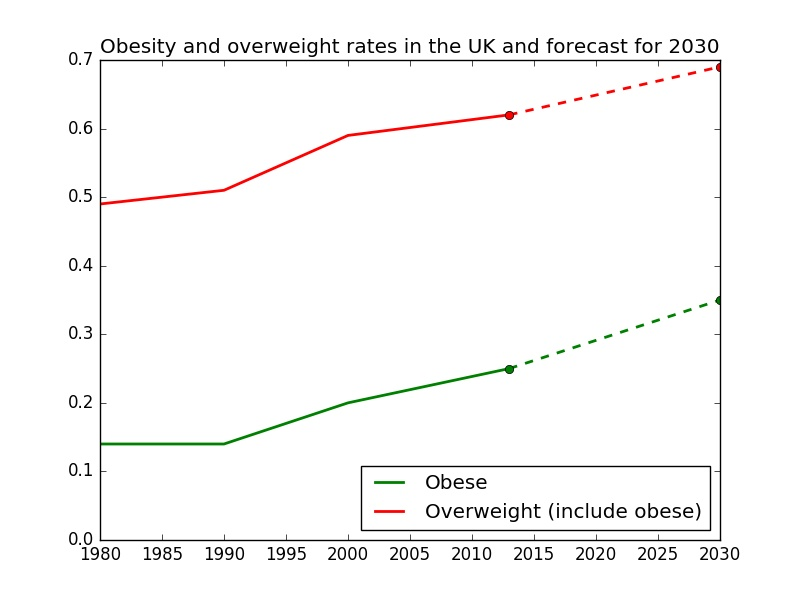
\includegraphics[width=0.5\textwidth,  height=0.455\textwidth ]{img/obesity_uk.jpg}
    \caption[Obesity and overweight rate of the adult population in the uk between 1980 and 2030. \textit{Source: World Health Organisation}]{Obesity and overweight rate of the adult population in the uk between 1980 and 2030}
    \label{fig:obesity_uk}
\end{figure}

Being “overweight” is defined as having a Body Mass Index (BMI) – a person's weight in kilograms divided by the square of his height in meters (kg/$m^2$) – of between 25 and 29.9, and “obese” by a BMI of 30 and above.

As stated in \cite{Mokdad2003}), obesity is strongly associated with several major health risk factors such as stroke, high blood pressure, type 2 diabetes and high cholesterol.

Diabetes:
- fast growing (current ... in to ... in) with forecast for ... to be ...
- lead to high mortality
- treatment cost. \cite{Zhang2010}: in 2010: 12 \% of the total whorlwide health expenditure is spent on diabetes and will continue to increase.

Combination of drugs and food intake control have shown great results

Main reason: junk food: easily found, cheap.

One of the best way to fight it: watch over what we eat. Associated lifestyle changes and lose weight. It can also be used as a prevention tool for population at risk

studies such as \cite{Burke2011a} show the benefit of reporting its daily diet to lose weight and improve the quality of its foos intake

Also a way to ... eat disorders

Currently, manually ... self reporting, using paper diaries : tedious + time consuming + prone to errors (users tend to underestimate its intake as describe in \cite{Lichtman1992}) + need a trained patient

At the same time, improvement of the classification methods. Imagenet, a 1000 classes and more than 1,2 million images dataset example on Image Net results \cite{Russakovsky2015}.
Every year since 2010
Numerous institutions (university, tech companies) are participated
As described in figure \ref{fig:imagenet_results}, the mean error for each class for classification and localization has been greatly reduced between 2010 and 2014

\begin{figure}[h]
    \centering
    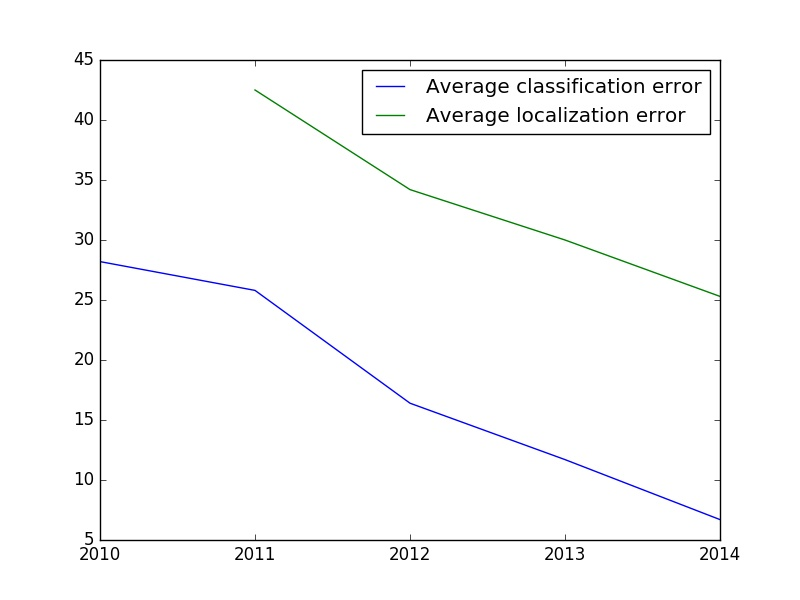
\includegraphics[width=0.5\textwidth,  height=0.455\textwidth ]{img/imagenet}
    \caption{Average classification and localization error of the best results for different ImageNet challenges}
    \label{fig:imagenet_results}
\end{figure}

Recently: proposition automize it. With the widespread use of smartphone, people can easily take pictures of a good quality. People are already taking picture of their food and posting them on website such as Food Gawker, Instagaram, Flickr, Yelp or 

That's why, over the past few years, people ... automated it. Assist patient and their medical personnel
Extends the reach of care in a cost effective ways and counters some of the previous problem (still pb with the elder / people who don't have access to smartphone). Or using weerable device to automatically take picture

Part of the rise of e-healthcare / m-healtchare \cite{Hillestad2005, Menachemi2011}

food recognition: promising applications of image processing and machine learning. Estimate food intake and people's habit

Overall process:
extract characteristic (possible features are invariant of the liminosity, orientation, scale, ...)segmentate, classify, get calorie value or a simplified version (using for example the ... systems), keep log and being able to visualize it over the year

Feature description: key to achieve good object detection and image categorization

In this thesis: focus on the first two phases

Already have numerous challenges:
large number of food items
variation in appearance and shape with numerous transformation can be applied to a same picture (scale, translation, rotation, skewness)
different way to serve it
environmental condition
--> lead to a high inter-class variability


The organization of this thesis is as follow. In section ..., previous work is reviewed. In section ..., I explain and describe the dataset choosen, then the different image descriptors and classifiers used. In the next section, we present and discuss our results. Finally, in section ..., the limitation and possible future work is discussed.


% show pictures as examples
